\documentclass[compress]{beamer}
\usetheme{Warsaw}

\usepackage[dutch]{babel}

\usepackage[utf8]{inputenc}
\usepackage{amsmath}
\usepackage{amssymb}
\usepackage{txfonts}
\usepackage{graphicx, import}
\usepackage{csquotes}
\usepackage[backend=biber, style=ieee]{biblatex}
\usepackage{pgfplots}
\usepackage{siunitx}
\usepackage{caption}
\usepackage{subcaption}
% \RequirePackage[left=2cm,right=2cm,top=2.2cm,bottom=4cm]{geometry}
% \RequirePackage[pdftex,pdfpagelabels,bookmarks,hyperindex,hyperfigures,hidelinks]{hyperref}
% \RequirePackage{listings}  % for code
\usepackage{xcolor} % needs to be after listings

\newcommand\ph{\mathrm{pH}}

\institute{HvA}
\date{\today}

\begin{document}

\title{pH meten met een ISFET}
\subtitle{Sensor modules}
\author[Tycho Jöbsis \and Jochem Leijenhorst \and Illya Ustenko]{
    {
        % \section*{\hspace*{l}}
        \begin{tabular}{ll}
            Tycho Jöbsis        & (500845792)\tabularnewline
            Jochem Leijenhorst  & (500855372)\tabularnewline
            Illya Ustenko       & (500845492)        
        \end{tabular}
    }
}

    \begin{frame}
        \titlepage
    \end{frame}
    
    \begin{frame}
        \frametitle{Inhoudsopgave}\tableofcontents
    \end{frame} 

    \begin{frame}
        \frametitle{Opdracht}

        % Elk ontwikkelteam gaat een eigen systeemontwerp bedenken en verder uitwerken: blokschema, circuitniveau, realisatie, en tenslotte metingen ter validatie.
    
        % % Elk ontwikkelteam bestaat uit 3 en soms 4 studenten en gaat zijn eigen systeemontwerp bedenken en verder uitwerken: blokschema, circuitniveau, realisatie, en tenslotte metingen ter validatie.

        % Per ontwikkelteam wordt tenminste 1 sensormodule gemaakt. De ontwikkeling en de validatie van de sensormodule en moeten tijdens de eindpresentatie overzichtelijk gestructureerd binnen de tijd worden gepresenteerd.

        \begin{itemize}
            \item Onderzoek naar drinkwaterproductie
            \item pH meten 
            \begin{itemize}
                \item Nauwkeurig
                \item Over langere tijd
                \item Naar bestaand base station
            \end{itemize}
        \end{itemize}

%         Voor het doen van onderzoek naar productiemethoden van drinkwater, het is belangrijk om tijdens verscheidene productie stappen de pH waarde van het water te kunnen meten. Om dat mogelijk te maken zal er in dit project gewerkt worden aan een eerste prototype van een pH sensormodule. Deze sensormodule zal rondom een ion gevoelige veld effect transistor (ISFET) worden ontwikkeld. De reden dat er geen gebruik gemaakt wordt van een glazen electrode pH sensoren is omdat deze duurder zijn om te produceren \cite{duroux1991ionpHISFETltspHmonitoring}. 

% In het onderzoek waar deze sensormodule voor wordt ontwikkeld, zullen er meerdere van deze modules voor langere tijd data verzamelen. Om het makkelijk te maken om de pH meetdata te verzamelen heeft de sensormodule een draadloze verbinding nodig. Via deze draadloze verbinding is het dan mogelijk om de meetdata naar een basisstation te sturen. Dit basisstation is al ontwikkeld. 

% Verder zal er gekeken worden naar methodes van energie harvesting om de levensduur van de sensormodule te verlengen. 

    \end{frame}

    \section{Systeem}

\subsection*{Diagram}


\begin{frame}
    \frametitle{Systeemdiagram}
    
    \only<1>{
        \begin{figure}
            \centering
            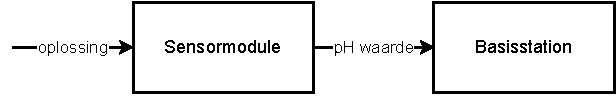
\includegraphics[width=\textwidth]{toplevelDiagram}
        \end{figure}
    }
    \only<2>{
        \begin{figure}
            \centering
            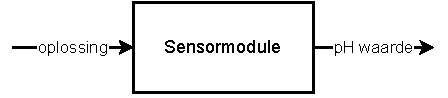
\includegraphics[width=\textwidth]{topLevelModuleOnly}
        \end{figure}
    }
\end{frame}

\transboxin


\begin{frame}
    \frametitle{Systeemdiagram}
    
    \begin{figure}
        \centering
        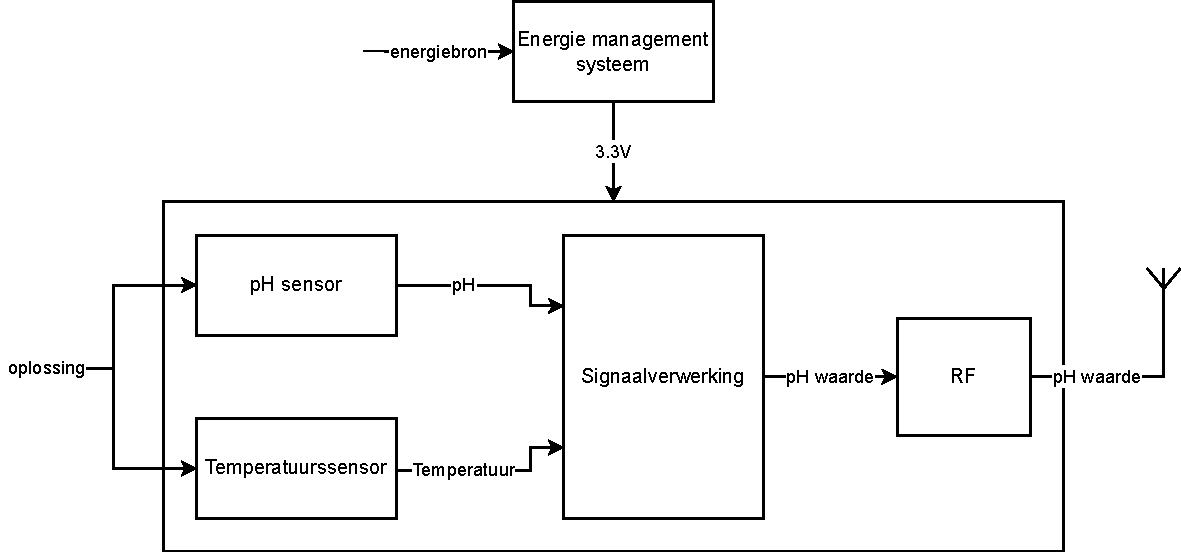
\includegraphics[width=\textwidth]{moduleDiagram.pdf}
    \end{figure}
    
\end{frame}



\subsection*{Eisen}
\begin{frame}
    \frametitle{Systeem eisen}

    \begin{table}[ht]
        \centering
        \begin{tabular}{|l|c c|l|}
            \hline
            Beschrijving                    & Min               & Max   & Eenheid           \\
            \hline 
            Afwijking                       &                   & 0.05  & pH                \\ 
            Bereik                          & 2                 & 10    & pH                \\
            Bandbreedte                     & 10                &       & Hz                \\
            $\mathrm{SNR}_{uit}$            & 36                &       & \qty{}{\decibel}  \\
            Rf afstand                      &                   & 10    & \qty{}{\meter}    \\
            Rf BER                          & $1\times10^{-5}$  &       &                   \\
            Levensduur                      & 48                &       & \qty{}{\hour}     \\
            Gemiddeld gebruikte vermogen    &                   & 10    & mW                \\
            Energy harvesting               & $>$ 0             &       & mW                \\
            \hline
        \end{tabular}
        \caption{Systeemspecificaties.}
        \label{tab:systemSpecs}
    \end{table}

\end{frame}
    
% \end{frame}
\subsection*{decompositie}
\begin{frame}
    \frametitle{Functionele decompositie}
%     \begin{figure}
%         \centering
%         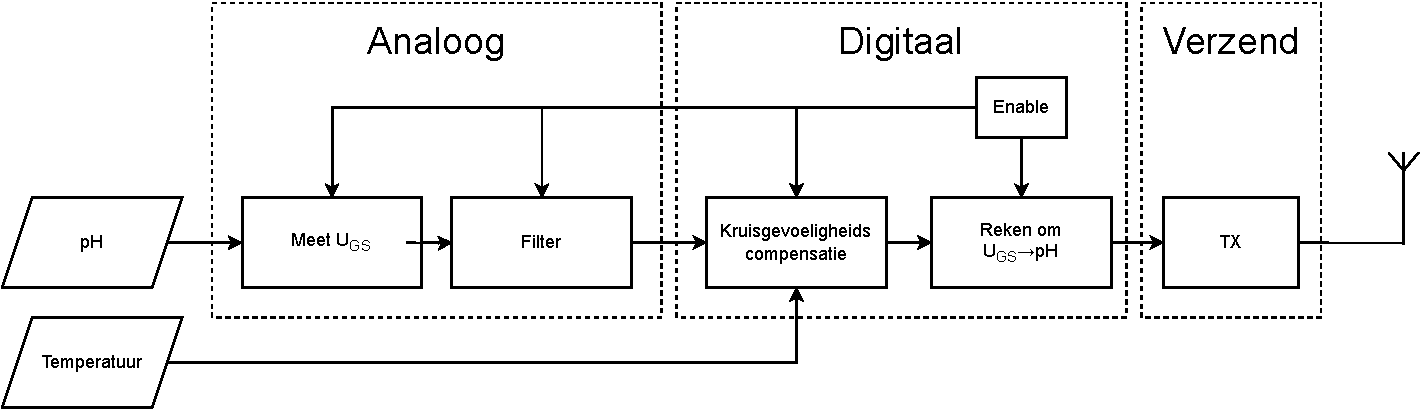
\includegraphics[width=\textwidth]{img/meetGedeelte.pdf}
%     \end{figure}
%     \begin{figure}
%         \centering
%         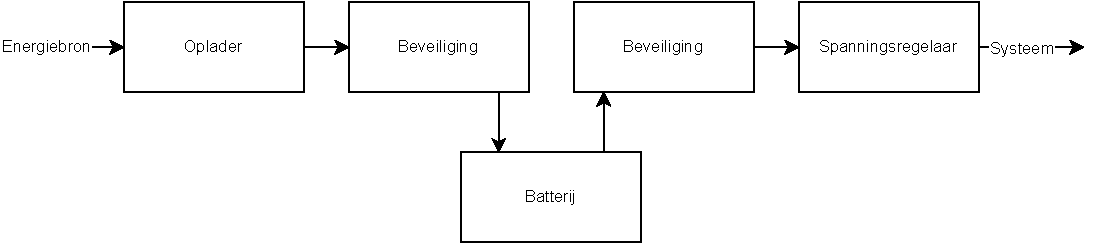
\includegraphics[width=\textwidth]{img/funcdDecompEnergy.pdf}
%     \end{figure}    
% \end{frame}
% \subsection*{Energie \& ruis}
% \begin{frame}
%     \frametitle{Energie \& ruisbudget verdelen}

%     SNR systeem uit = 34dB

%     \begin{table}
%         \centering
%         \begin{tabular}{l|l|l}
%             Func. blok          & Vermogen [mW] & NF [dB]   \\\hline
%             Reken $U_{GS}\rightarrow$pH & 0.6   & 3         \\
%             ADC                 & 1             & 3         \\
%             AA-filter           & 0.2           & 3         \\
%             Meet $U_{GS}$       & 0.2           &           \\\hline
%             Zenden              & 5             &           \\\hline
%             Oplader             & 0.5           &           \\
%             Beveiliging         & 0.5           &           \\
%             Spanningsregeling   & 1             &           \\ 
%         \end{tabular}
%     \end{table}

%     \pause

%     SNR Meet $U_{GS}$  $>43$dB

\end{frame}
    
    \section{pH meten}
    \subsection*{pH meettechnieken}
    \begin{frame}
        \frametitle{pH meettechnieken}
    
        \begin{itemize}
            \item pH-meetstrip
            \item ISFET
            \item Glas-probe
        \end{itemize}
    
    \end{frame}

    \subsection*{ISFET informatie dragend signaal}
    \begin{frame}
        \frametitle{ISFET informatie dragend signaal}

        De threshold spanning is afhankelijk van de pH.

        Met constante $U_{DS}$ en $I_{DS}$ is $U_{GS}$ lineair afhankelijk van de pH.
    
    
    \end{frame}

    \section{Sensor data naar pH omzetten}

\subsection*{Uitlezen ISFET}

    \begin{frame}
        \frametitle{Principe schakeling}
    
        \begin{figure}
            \centering
            \def\svgwidth{0.6\textwidth}
            \input{ISFETCircuitBest.pdf_tex}
        \end{figure}
    
    \end{frame}
    \begin{frame}
        \frametitle{Ruis analyse}
    
        \begin{figure}
            \centering
            \def\svgwidth{0.6\textwidth}
            \input{ISFETCircuitBestNoise.pdf_tex}
        \end{figure}
        \begin{equation}\label{eq:measureNoiseOut}
            S_{u_{{n,out}}} = \left(S_{u_{{n,ref}}} + S_{u_{{n,n}}} + S_{i_{{n,in}}}\left(Z_{fet} // R\right)^2\right) \cdot H^2(\ph)
        \end{equation}
    
    \end{frame}
    \begin{frame}
        \frametitle{Energie}

        $U_{dd}=3v3$

        \noindent
        $I_{ds}=50\mu$A
    
        \begin{equation}\label{eq:measurePower}
            P_{statisch} = P_{n,quiescent} + U_{dd}I_{ds}
        \end{equation}

        \pause

        \begin{equation}
            P_{statisch} = P_{n,quiescent} + 165\mu\mathrm{W}
        \end{equation}
    
    \end{frame}

    \subsection*{ADC}
    \begin{frame}
        \frametitle{Eisen}
    
        \begin{table}[ht]
    \centering
    \begin{tabular}{l|c|l}
        Symbol      & Waarde & Eenheid\\\hline
        $SNR_{in}$  & 37        & dB\\
        NF          & 3         & dB\\
        $u_{in}$    & 2.5       & mV\\
    \end{tabular}
    \caption{De eisen voor het omzetten van het analoge signaal naar een digitaal signaal.}
    \label{tab:systemSpecADC}
\end{table}
    
    \end{frame}
    \begin{frame}
        \frametitle{Minimum aantal bits}
        \centering

        De toelaatbare fout ten gevolge van de eindige resolutie van de ADC
        \begin{equation}\label{eq:calcSpecifiedRmsError}
            \overline{e_{eff}^2}=\left(10^{\frac{NF}{10}}-1\right)\left(\frac{S_{rms}}{10^{\left(SNR+NF\right)/20}}\right)^2
        \end{equation}
        \pause

        Berekenen minimum benodigde ADC resolutie
        \begin{equation}\label{eq:calcNeededQ}
            Q=\sqrt{12\cdot\overline{e_{eff}^2}}
        \end{equation}
        \pause

        Berekenen minimum aantal bits van de ADC op basis van de minimaal benodigde ADC resolutie 
        \begin{equation}\label{eq:calcMinNumberADCbits}
            n=\left\lceil\log_2\left(\frac{1}{Q}+1\right)\right\rceil=14
        \end{equation}
    
    \end{frame}

    \begin{frame}
        \frametitle{Sample frequentie}
        \centering
        
        Toelaatbare fout
        \begin{equation}\label{eq:ADCmaxSampleError}
            E=10^{\frac{-NF}{10}}
        \end{equation}
        \pause

        Minimale sample frequentie berekenen
        \begin{equation}\label{eq:ADCminFs}
            f_{s,min}=\frac{\pi f_h}{E}=45
        \end{equation}
    
    \end{frame}

    \subsection*{AA filter}
    \begin{frame}
        \frametitle{Eisen anti aliasing filter}
        
        \centering

        Dempen 22.5Hz


        $P_{max}=200\mu$W


        $NF=3\si{\decibel}$

        %TODO! Voeg hier een afbeelding van een RC filter
        [Voeg hier een afbeelding van een RC filter]
    
    \end{frame}
    \begin{frame}
        \frametitle{Ruis \& vermogensanalyse RC filter}
    
        \begin{equation}\label{eq:dividerNoise}
            u_{n,out}^2 = \frac{kT}{C}
        \end{equation}

        \begin{equation} \label{eq:filterPower}
            P = \frac{1}{\sqrt{2}}\omega_cCU_{in,max}^2
        \end{equation}

        \pause

        \begin{equation} \label{eq:filterCapMin}
            C_{min} = \frac{kT}{u_{n,in}^2}
        \end{equation}

        \begin{equation}
            R = \frac{1}{2\pi fC}
        \end{equation}
    
    \end{frame}
    \begin{frame}
        \frametitle{AA filter}
    
        \begin{table}[ht]
            \centering
            \begin{tabular}{l|l|l}
                Symbool & Waarde & Eenheid \\
                \hline
                $C$         & 82    & $\si{\nano\farad}$\\
                $R$         & 180   & $\si{\kilo\ohm}$  \\
                $f_c$       & 10.8  & $\si{\hertz}$     \\
                $P$         & 408   & $\si{\nano\watt}$ \\
                $u_{n,out}$ & 225   & $\si{\nano\volt}$ \\
                NF          & 0.23  & $\si{\decibel}$   \\
            \end{tabular}
            \caption{De gekozen waardes van het filter, en de resulterende vermogens- en ruiseigenschappen.}
            \label{tab:filterValues}
        \end{table}
    
    \end{frame}
    \begin{frame}
        \frametitle{Effecten van de load}
    
        Spanningsdeler met de ADC, hierdoor wordt het ingangssignaal kleiner.
    
    \end{frame}

    \subsection*{Berekenen pH}
    \begin{frame}
        \frametitle{Gemeten waarde omrekenen naar pH}
        
        %TODO jochem doe werk/voeg dingen toe
        % $\mathrm{CAL_{\mathrm{pH,H}}}=7$

        % $\mathrm{CAL_{\mathrm{pH,L}}}=4$

        % \begin{equation}
        %     \mathrm{pH}=\frac{\mathrm{S}-\mathrm{CAL_{\mathrm{ADC,L}}}}{\mathrm{CAL_{\mathrm{ADC,H}}}-\mathrm{CAL_{\mathrm{ADC,L}}}}\left(\mathrm{CAL_{\mathrm{pH,H}}}-\mathrm{CAL_{\mathrm{pH,L}}}\right)+\mathrm{CAL_{\mathrm{pH,L}}}
        % \end{equation}
    
    \end{frame}

    % # Ontwerp
% ## ...
% ##


\subsection{De oplaadbare voeding van het systeem} \label{sec:energy}

De sensormodule heeft energie nodig om te functioneren. Deze energie moet geleverd worden door een energie management systeem in de vorm van een constante spanning. Het voedingsblok ligt buiten het signaalverwerkingspad, zoals te zien is in \cref{fig:moduleDiagram_energie}.

\begin{figure}[!htb]
    \centering
    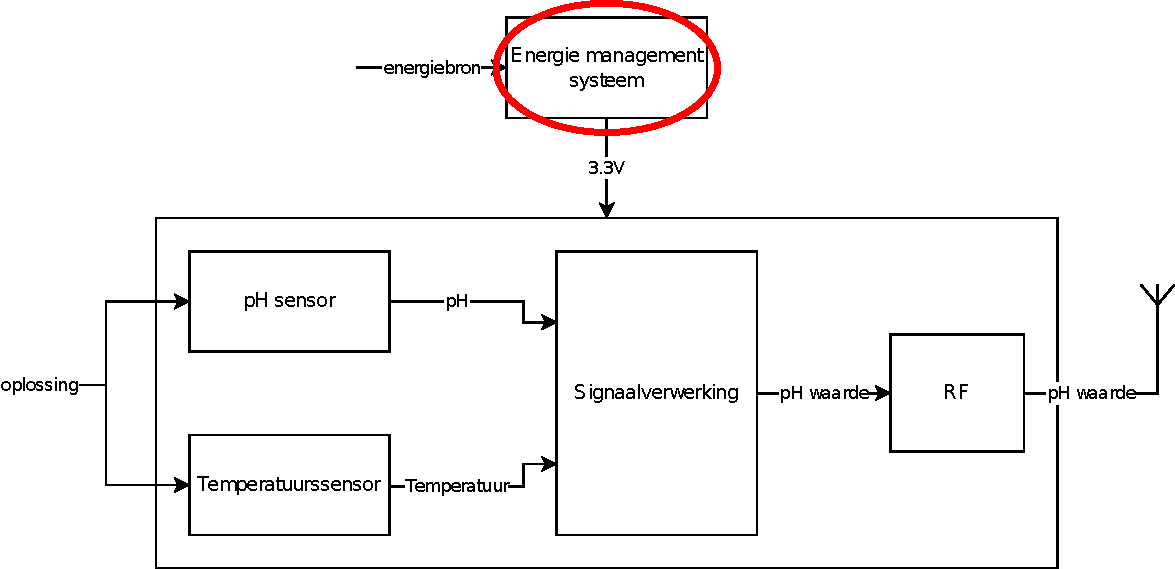
\includegraphics[width=.7\textwidth]{moduleDiagram_energie}
    \caption{De locatie van het energie management systeem in het blokschema van de sensormodule.}
    \label{fig:moduleDiagram_energie}
\end{figure}

Het energie management systeem moet energie kunnen opnemen uit de omgeving, en dit kunnen opslaan. Hiervoor zijn een energy harvesting systeem en een accu nodig.

\subsubsection{Energy Harvesting} \label{sec:harvesting}

Vanuit de opdrachtdefinitie is er gekozen voor een piëzo-element. Deze piëzo kan mechanische trillingen omzetten naar elektrische energie. Deze energie kan gebruikt worden om de accu op te laden of het energieverbruik van de module te verminderen.

Een piëzo-element produceert energie in de vorm van wisselspanning. Deze spanningen kunnen oplopen tot spanningen boven de \qty{20}{\volt}.% TODO: bron????
Hierdoor zal er, naast een gelijkrichter en een spanningsregelaar, ook een beveiliging tussen het piëzo-element en de rest van het systeem geplaatst moeten worden.


\subsubsection{Accu} \label{sec:batterijOntwerp}
Er zijn veel verschillende soorten soorten oplaadbare batterijen die gebruikt kunnen worden bij een sensor module.
Voor de type sensor module waar dit verslag over gaat is gekeken naar 4 verschillende oplaadbare accu opties\cite{battery-comparison}:

\begin{enumerate}
    \item Lithium-Ion (Li-Ion)
    \item Lithium Polymeer (Li-Po)
    \item Zebra (Zout nickel)
    \item Nickel-Cadmium (Ni-Cd)
\end{enumerate}

In onderzoek \cite{battery-comparison} is het duidelijk aangetoond dat Li-Po het hoogste energiedichtheid heeft. Dit zou een praktische overweging zijn om de sensor module compact te houden. Dit heeft ervoor gezorgd dat voor de sensor module ontwerp een LiPo gekozen is als batterij. Spanning van een cel (1s) LiPo is maximaal \qty{4.2}{\volt} en minimaal veilige spanning is \qty{2.7}{\volt}\cite{BatteryComparison}. Dit is een van de specificaties van de batterij management systeem.


\subsubsection{Voeding} \label{sec:voeding}
De voedingsspanning is gekozen vanuit de maximale spanning die nodig is voor de ISFET sensor\cite{isfet}. Hieruit volgt een maximale systeemspanning van \qty{3.3}{\volt}.

Zoals te lezen in \cref{sec:batterijOntwerp} is er gekozen voor LiPo batterij technologie. De batterij heeft een beveiliging voor beide op- en ontladen nodig. De celspanning moet omgezet worden naar systeemspanning van \qty{3.3}{\volt}. Dit kan op meerdere manieren gedaan worden. Twee hiervan zijn een DC-DC buck-boost converter en een low dropout regelaar (LDO). De buck-boost converter is efficiënter dan de LDO, maar heeft een minder stabiele uitgang. Hierdoor is ervoor gekozen om beide soorten regelaar te gebruiken. Dit is te zien in \cref{fig:voedingSchematisch}. Het digitale gedeelte van het systeem wordt gevoed door een buck-boost converter; de spanningsrimpel van de buck-boost converter maakt minder uit voor een goed ontkoppelde microcontroller.
De uitgang van de buck-boost converter wordt vervolgens gestabiliseerd door een LDO, die het analoge gedeelte van het systeem voedt. De uitgangsspanning van de LDO zal iets lager zijn dan de uitgang van de buck-boost converter, wat geen problemen zal vormen zolang het verschil minimaal is.

Zoals beschreven in \cref{sec:harvesting} moet de uitgang van het piëzo-element gelijk gericht en beschermt worden. In \cref{fig:voedingSchematisch} wordt het gelijkrichten gedaan door de AC-DC omvormer.

Voor energy harvesting is er een piëzo-element gekozen. Een piëzo-element kan gezien worden als een AC bron. Deze AC bron moet omgezet worden naar DC die door het systeem gebruikt kan worden om de batterij mee op te laden. De AC bron wordt met een gelijkrichter naar DC omgezet. Deze DC spanning is niet hetzelfde als de systeemspanning dus die moet omgezet worden naar een spanning die de batterij in gaat, zodat de batterij kan opladen.

\begin{figure}[!htb]
    \centering
    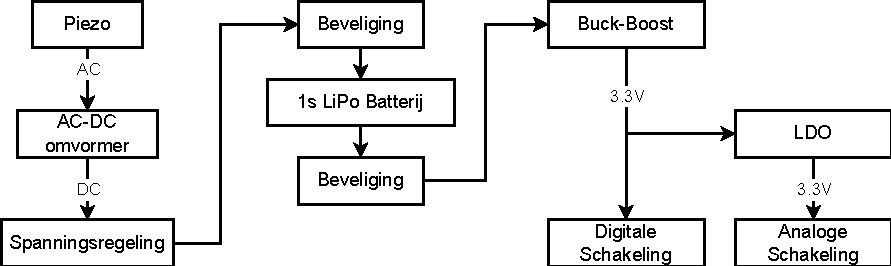
\includegraphics{voedingSchematisch.pdf}
    \caption{Voeding schematisch}
    \label{fig:voedingSchematisch}
\end{figure}



\subsubsection{Energie budget}\label{sec:energyBudgets}
Voor het energiebudget zijn de waardes in \cref{tab:energieBudgetEstimatie} gekozen. Elk van deze waardes ligt boven het theoretisch berekende minimum van het respectievelijke systeemonderdeel. De som van de vermogens is \qty{9}{\milli\watt}, wat onder het maximale toegestane energieverbruik van \qty{10}{\milli\watt} ligt.


\begin{table}[!htb]
    \centering
    \begin{tabular}{l|l}
        Func. blok          & Vermogen [mW] \\
        \hline
        Reken $U_{GS}\rightarrow$pH & 0.6   \\
        ADC                 & 1             \\
        AA-filter           & 0.2           \\
        Meet $U_{GS}$       & 0.2           \\
        Zenden              & 5             \\
        Oplader             & 0.5           \\
        Beveiliging         & 0.5           \\
        Spanningsregeling   & 1             \\
        \hline
        \hline
        Totaal              & 9

    \end{tabular}
    \caption{Energie budget}
    \label{tab:energieBudgetEstimatie}
\end{table}




    % \section{Vragen}
    \begin{frame}
        \frametitle{Vragen?}
        
        \centering
        Zijn er nog vragen?
    
    \end{frame}

\end{document}